\chapter{Achievements}
\par This part will a melting pot of issues and success and how I found out how to correct them if I could. I will gather the installations for OpenCV and the cross toolchain because the main idea is the same. Then I will spit the technical part in two as usual otherwise it will not be clear enough.	
	
	\section{Installation and tests}
	
	\subsection{Helmet}
	\subsubsection{Cross GCC}
	
	\par It is pretty easy to install, you have to get the archieve and compile the cross compiler for your architecture. First of all I saw in the tutorial required a Ubuntu 12.10LTS\footnote{Long Lime Support} at least. I used virtual box to get a virtual machin\footnote{Software to emulate operating systems} of this distribution on my windows operating system. Next, I simply followed the tutorial that explains how to install the cross compiler. This part was really easy, after have download GNU cross G++ I ran commands and the compiler was installed.
	
	\subsubsection{Kernel compilation}
	
	\par The compilation of the kernel is almost the same as the compiler itself except that you compile for another platform. Of course the compiler handle ARM cortex A8 for TI OMAP3 otherwise. I just had to check the option for this CPU\footnote{Central processing unit} during the installation and thant the kernel I compiled was compatible with this architecture. As a result I got a file system ready to boot on an ARM device.
	
	
	\subsubsection{Tests}
	
	\par Once the file system is compiled, I had to put it inside the helmet memory. Two main problems remained, first the helmet memory was inside the helmet itself and not in the memory stick. And secondly, you can only copy files using Windows CE on the intern memory. This means that you can not erase Windows CE file system and replace it by another.
	\par That is were I found out that the project was compromised. I had few knowledges in Windows CE and the fact the helmet was not booting at first and the interface is voice commanded. I estimated the time to solve the problem longer than my internship.
	\par Thus I tryed to launch the file system on qEmu which failed. When I explained all of that to my superior they decided to change the project.
	
	\subsection{Pattern scanner}
	\subsubsection{OpenCV installation}

	\par I installed OpenCV 3.0 which is the last version and tried it. It has a base for basic image applications and modules that you can install by adding them to the module folder and compile them. Unfortunatly one module required to perform the test was not working with the 3.0 version. It is the non free module. I tryed several times but I finally decided to switch back to a previous version. After uninstall everything and install the 2.4.9 version. The module was functionnal. I tryed the code of the tutorial ~\hyperlink{opencv}{I quote earlier} and I had the first pattern recognition result. That took me 4 day in totall including the eclipse configuration that require adding all the libraries in the configuration of the compiler.
	
	\subsubsection{First build on eclipse}	
	
	\par As I just said, to make it work on eclipse I had to set the configuration for OpenCV project. Otherwise I does not compile. Right click on the project, propreties, than	go to the settings of my compiler (GCC  C++) and select includes. There I added the path to the local install folder where the OpenCV's includes are located. After that I had to set the libraries to link one by one. In the same window I went in libraries section and add their names like opencv\_core... And I added the search path of my local lib folder. Then I saved the setting and compilation was working.
	
	
	\section{Main problems}	
	\subsection{Related to the helmet}
	\par I had several issues before I began working proprely on the helmet. Some of them are related to the hardware and others to the operation system.
	\subsubsection{Hardware}
	\par The first problem we encountered was getting access to the component references of the helmet like processor, camera, mother board, etc. Pierluigi, my tutor sent mails to the company which proposed the project. Unfortunatly they was not able to gain access to this information. I looked it on the manuals and documentation that Pierluigi gave to me and the Internet. Everytime, I couldn't get the precise references, only the names of the range of the product are available.

	\par Besides, there was little issues with the helmet itself because the alimentation module was missing. That module allows us to plug the helmet directly to the outlet. To resolve the problem I had to load the batteries and plug it to the helmet to boot it.

	\subsubsection{Emulator}
	
	\par I download and install easily the emulator (qEmul) advised in the tutorial that I followed but I couldn't run the operating system on  it. The operating system started on a black screen and then nothing happend. I did not find a solution to this problem because I found out that the project was already compromised by the fact that we did not have access to the references of the components. Still I was a little bit suprised that the emulation was not working because all the steps of the tutorial was working except this one.
	
	\subsubsection{The operating system}
	
	\subsection{Related to the software}
	
	\subsubsection{The matcher}
	
	\par After 3 days of stagnation making some tests and learing about the matching system. Allessia, the thesis companion of Mario Vento made me realise that was on the wrong way using the match function of OpenCV. In fact I couldn't find multiple pattern with that method because it selects the nearest descriptors\footnote{Those which have a minimum hamming distance likeness}. The result was that I had to launch serval time the algorithm to get new matches again and again. I found the knnmatcher that perform a full matching and keeps the N best matches. That was not enough so I switched to the radius matcher that need a threshold parameter. That it finally how I introduce the threshold in the program. This value depends on the object, the distance and the conditions of the scene. In an other way the matcher keeps the matches which differ between the scene and the pattern less than the threshold.
	\par The algorithm return a vector of vector of DMatches\footnote{DMatch : A structure representing each match} so I put it in a simple vector of DMatches and it gave me very good results. The algorithm was able to find multiple time the same match on the scene. In the figure \ref{matches} we can see the fact that every time the pattern is represented it has matches in it. Not just the best ones which here corresponds to those of the first on the left.
	
	
	\begin{figure}[h]
		\begin{center}
			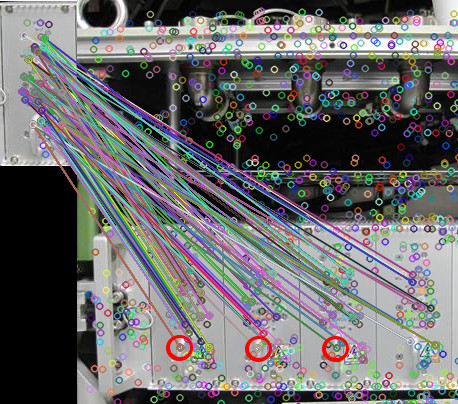
\includegraphics[width=10cm]{images_not_compressed/matches.jpg}
			\caption{Simple draw of radius match with 3 times the same match surround in red}
			\label{matches}	
		\end{center}
	\end{figure}
	
	\subsubsection[Multiple pattern]{Get many time the same pattern}

	\par On this part we extract two possible methods with Pierluigi. The easy one was to draw in black the image and than make the homography another time. The hardest one was to look for the key points and descriptor inside the corners and earase them of their containers. Than do the homography again. I began by the second one that sounded more relevent. 
	
	\par To be clear I have to present the DMatch structure that is detailed in the \hyperlink{structDMatch}{annexes}. The important attributs are the train index and the query index. They represent the fact that a descriptor has been found on the two images. But only the index of the descriptor is stored.
	
	\par I first thought I could get easily the points that gave me the corners after the homography. In fact I needed to remove the points that concern the pattern that has been recognized by the homography. There was no other way but to extract all the indexes of the points inside the corners I just found and remove them from the vectors. By chance, the homography take to vectors of points describing the positions of the descriptors (and the key points by the way). 
	\par On the first version of this algorithm I was looking if the point was in the bounds represented by the 4 segments of the rectangle of the pattern found. I found out when I was rotating the image that the points was removed the wrong way because the shape of the pattern was a lozenge. A lot of points was concidered out of the bounds and other that had nothing to do with the pattern was removed.
	\par I found on the internet a method~\cite{InOut} that provides the answer of my problem in O(n). This method find the number of edges that ligne from a point cross to the infinite with a polygon. If it is odd then the point is inside the polygon otherwise it is outside. The picture~\ref{OutIn} illustrate the idea.
	\begin{figure}[h]
		\begin{center}
			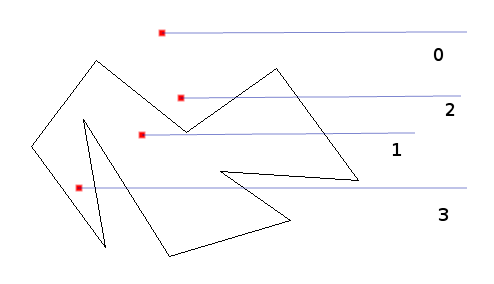
\includegraphics[width=10cm]{images_not_compressed/isIn.png}
			\caption{Illustration of the algorithm that tell if a point is inside a polygon}
			\label{OutIn}	
		\end{center}
	\end{figure}
	\subsubsection{Corners}
	\par OpenCV does not implement a structure for the corners. The corners correspond to the vertices of the polygone that represents the pattern. I isolated them in the first place beaucoup that is a good proof of the fact that the algorithm found efficiantly a pattern. It also helped me to find out that the first version of the removing point algorithm was not working perfectly.
	\par I let the structure as it is because I told myself that, in the future, the application could need the corners of the pattern to compute move analysis for exemple. 	
	
	\subsubsection{Others}
	
	\par My biggest parallel achivement is an algorithm that helps the user of the application to find the best threshold for his patterns. It depends of the number of pattern you want to recognize because often the threshold must be higher for certain conditions and more there is pattern in the image, more there is different conditions. 
	\par The algorithm take a scene and a pattern in input plus the number of time the pattern is represented in the image. The result of the algorithm is the first threshold that got all the patterns in the image. It computes a range of 150 values, that is why I can take 2 or 3 secondes sometimes.
	
	\begin{figure}[h]
		\begin{center}
			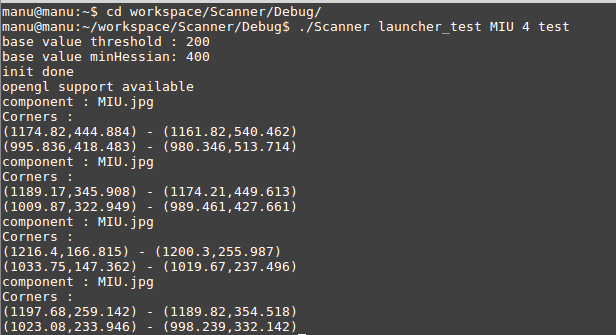
\includegraphics[width=10cm]{images_not_compressed/tester.png}
			\caption{Screenshot of the algorithm finding four times the MI unit pattern}
		\end{center}
	\end{figure}	
	
	\par We can see here that for units has been found with the positions of there corners
	
	\par I also had to create a video for Pierluigi to show case the possibilities of my application. Therefore I used VLC media player to stream my screen during a demonstration. I turned the stream into mp4 and used Kdenliv to make some modification and add titles. When the result was good enough I used GNOME Subtitles to write an .str file that corresponded to the video. Then I uploaded the video on youtube to share it with Pierluigi. I made some changes in the begining of the video several times. That took me a long time because I had to change manually all the subtitles that passes after the adding or the suppression.
	\par the video is accessible here : \url{https://youtu.be/q23RjtwAqDU} you can see in the figure ~\ref{video} the page were I edited the proprety and added the subtitles to make it available on youtube.
\begin{figure}[h]
		\begin{center}
			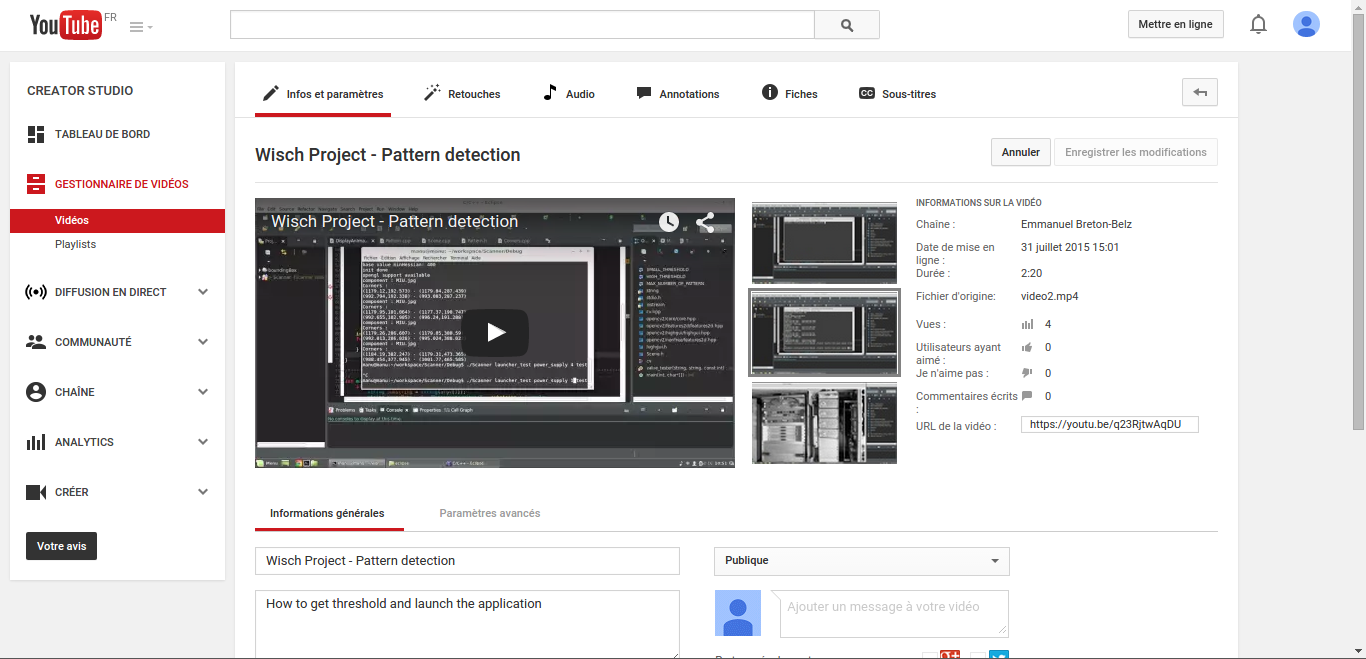
\includegraphics[width=10cm]{images_not_compressed/screenShot.png}
			\caption{Youtube edition page of the video}
			\label{video}	
		\end{center}
	\end{figure}	